\chapter{Grafo PTN}
\label{cap2}

Per analizzare le caratteristiche complesse della PTN, bisogna prima costruire e rappresentare la rete. Il modo migliore per rappresentarla è attraverso un \textbf{grafo}, le cui caratteristiche saranno meglio approfondite nel corso di questo capitolo.

\section{Struttura PTN}
In un approccio generale, si potrebbe voler considerare un modello dinamico della PTN includendo capacità di carico dei convogli e delle linee, numero di passeggeri delle tratte e frequentazione degli itinerari insieme ad una visione completa della struttura PTN, ovvero le caratteristiche \textbf{topologiche} e \textbf{connettive} della rete \cite{vonFerber2012LondonParis}. \\
In assenza dei dati necessari per un simile approccio, questo studio si restringe all'analisi della struttura PTN, con l'obiettivo di studiare le caratteristiche strutturali, per poi analizzare il comportamento, in termini di \textit{resilienza} e \textit{vulnerabilità}, rispetto a determinate condizioni di \textit{stress strutturale}.

\section{Modello PTN}
L'osservazione che i percorsi di una città formino una \textbf{rete} è applicata da secoli, basti pensare all'utilizzo della \textit{teoria dei grafi} per risolvere il \textit{Problema dei ponti di Königsberg}.

\vspace{1em}
\begin{figure}[h!]
    \centering
    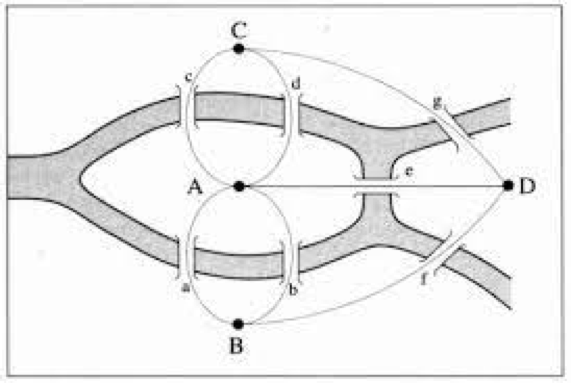
\includegraphics[width=0.4\linewidth]{Immagini//Capitoli//cap2/ponti.png}
    \caption{Grafo del problema dei ponti di Königsberg}
    \label{fig:Rappresentazione a grafo del problema dei ponti di Königsberg}
\end{figure}
\vspace{1em}

Ma che queste reti siano anche \textbf{complesse} è un concetto che si forma in tempi più moderni, con l'aumentare della complessità dei trasporti. Le \textbf{reti complesse} sono diventate recentemente il nucleo di un nuovo campo della conoscenza \cite{vonFerber2012LondonParis} che affonda le proprie radici nella \textit{teoria dei grafi} e nella \textit{statistica}.

\subsection{Modellazione come grafo complesso}
Da un punto di vista puramente matematico, una \textit{rete} non è altro che un \textbf{grafo} $G$ definito da un insieme $V$ di \textit{vertici} e un insieme $E$ di archi che collegano coppie di vertici.

$$
G = (V, E)
$$

Numerose strutture naturali e artificiali possono essere descritte in termini di \textit{grafi}, ma posseggono proprietà differenti da quelli che vengono chiamati \textit{grafi classici}. Tali reti sono classificate come \textbf{reti complesse}. \\
Alcuni esempi sono i sistemi biologici, gli ecosistemi, le reti sociali o le \textit{reti artificiali} come quelle di comunicazione o \textbf{di trasporto}.

Le reti complesse sono strutture \textit{compatte}, a volte definite \textit{piccoli mondi}, con poca distanza tra i nodi, un alto livello di correlazione e auto-organizzazione. Dimostrano resilienza rispetto ad attacchi casuali, d'altra parte hanno dimostrato anche una particolare vulnerabilità rispetto agli attacchi mirati dove con \textit{attacco} si intende la perdita di nodi o archi della rete.

\subsection{Modellazione in L-Space}
Per analizzare le varie proprietà di una PTN si deve iniziare dal modellare correttamente la \textit{topologia} della rete. Due delle modalità più usate sono chiamate $\mathbb{L}$-space e $\mathbb{P}$-space.

\vspace{1em}
\begin{figure}[h!]
  \centering
  % --- Prima immagine (a) ---
  \begin{subfigure}[b]{0.2\textwidth}
    \centering
    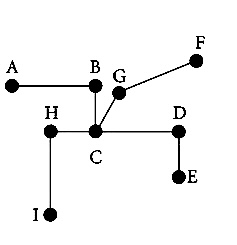
\includegraphics[width=\textwidth]{Immagini/Capitoli/cap2/L-space.jpg}
    \caption{}
    \label{fig:a l-space}
  \end{subfigure}
  \hspace{0.1\textwidth}
  % --- Seconda immagine (b) ---
  \begin{subfigure}[b]{0.3\textwidth}
    \centering
    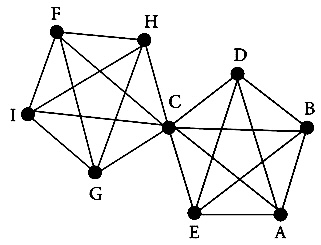
\includegraphics[width=\textwidth]{Immagini/Capitoli/cap2/P-space.jpg}
    \caption{}
    \label{fig:b p-space}
  \end{subfigure}
  % --- Didascalia generale ---
  \caption{Confronto tra una rappresentazione in $\mathbb{L}$-space (a) e $\mathbb{P}$-space (b).}
  \label{fig:confronto L-space P-space}
\end{figure}
\vspace{1em}

In questo studio si è usata la rappresentazione in figura \ref{fig:a l-space} perchè è quella che riproduce più fedelmente la \textit{topologia reale} della PTN. Tale rappresentazione $\mathbb{L}$-space consiste in un insieme di nodi che rappresentano \textit{fermate} e archi che rappresentano un \textit{collegamento} tra due fermate che esiste \textit{se e solo se} sono due fermate consecutive in almeno un \textit{percorso} \cite{vonFerber2012LondonParis}.

Il grado di ogni nodo in questa rappresentazione non è altro che il numero di direzioni \cite{SienkiewiczHolyst2005} che si possono intraprendere dal nodo stesso.

\section{Costruzione del grafo PTN}
Spostandosi su un punto di vista implementativo, il grafo relativo alla PTN in studio è stato costruito con l'ausilio della libreria \textbf{igraph} \cite{igraph} in Python, seguendo la struttura definita in figura \ref{fig:data integration} e costruendo quindi prima i nodi della rete e poi i vari collegamenti, rispettando le relazioni presenti nel dataset dei \textit{Trips}.

\subsection{Costruzione dei nodi}
Per evitare di includere nodi non presenti in alcun percorso, si sono costruiti a partire da una lista univoca dei nodi presenti in \textit{Trips}, acquisendo poi gli attributi dal dataset degli \textit{Stops}. Ogni nodo costruito presenta quindi la seguente struttura:
\begin{itemize}
    \item \texttt{name} id univoco numerico della fermata
    \item \texttt{stop-name} nome della fermata
    \item \texttt{longitude} longitudine della posizione geografica
    \item \texttt{latitude} latitudine della posizione geografica
    \item \texttt{lines} insieme di linee che transitano per la fermata
\end{itemize}

\subsection{Costruzione degli archi}
Per ogni percorso presente in \textit{Routes}, è stata ricostruita la sequenza di nodi appartenenti al percorso con il dataset \textit{trips}. Ogni arco costruito presenta quindi la sequente struttura:
\begin{itemize}
    \item \texttt{edges} coppia di nodi ai vertici dell'arco
    \item \texttt{lines} insieme di linee che transitano sull'arco, nella PTN in studio ogni arco corrisponde ad una sola linea, ma per generalizzare la struttura si è mantenuta comunque la possibilità di assegnare un arco a più linee
\end{itemize}

\subsection{Ridenominazione dei nodi}
Come evidenziato nell'analisi del dataset nella sezione \ref{subsec: analisi del dataset dellef ermate} alcune fermate, quindi alcuni nodi, pur essendo lo stesso nodo sono stati identificati in modi diversi a seconda della linea che servono. Per questa ragione, tali nodi presenti in \ref{tab:Ridenominazione di nodi con doppia identificazione} sono stati fusi in un solo nodo.

\vspace{1em}
\begin{table}[h!]
\centering
\begin{tabular}{lll}
\hline
\textbf{Nuova denominazione} & \textbf{Denominazioni precedenti} \\
\hline
Loreto &  Loreto M2, Loreto M1 \\
Cadorna & Cadorna FN M1, Cadorna FN M2\\
Duomo &  Duomo M1, Duomo M3 \\
Lotto &  Lotto FieraMilanoCity, Lotto M5\\
San Ambrogio &  S.Ambrogio, San Ambrogio \\
\hline
\end{tabular}
\caption{Ridenominazione di nodi con doppia identificazione}
\label{tab:Ridenominazione di nodi con doppia identificazione}
\end{table}
\vspace{1em}